\documentclass[11pt, twocolumn]{article}
\usepackage[T1]{fontenc}
\usepackage{amsmath, amssymb}
\usepackage{mathtools}
\usepackage{graphicx}
\usepackage[utf8]{inputenc}
\usepackage{fdsymbol}
\usepackage{textgreek}
\usepackage{natbib}
\usepackage{hyperref}
\usepackage{nameref}
\usepackage{url}
\usepackage{array}
\usepackage{csquotes}
\usepackage{caption}
\usepackage{algpseudocode}
\usepackage[a4paper, total={6.5in, 9in}]{geometry}
\usepackage[toc,page]{appendix}
\DeclarePairedDelimiter\floor{\lfloor}{\rfloor}
\providecommand{\myceil}[1]{\left \lceil #1 \right \rceil }
\hypersetup{
    colorlinks,
    citecolor=black,
    filecolor=black,
    linkcolor=black,
    urlcolor=black
}

\title{Decentralized state machine using Nakamoto (probabilistic) consensus\\\medskip Research Project 2022}
\author{Nicolas COURAUD (nicolas.couraud@etu.emse.fr)\\École Nationale Supérieure des Mines de Saint-Étienne}

\begin{document}

\maketitle
\onecolumn
\section*{Abstract}

As defined by Schneider \cite{stateMachine}, the state machine approach is a general method for implementing a fault-tolerant service
by replicating servers and coordinating client interactions with server replicas.

In this article, we will look at a new family of probabilitic consensus algorithms, in the context of building a decentralized state machine.

We will show that it is possible to build a decentralized state machine using Nakamoto Consensus, with the Snowball protocol \cite{snowprotocol} and will compare this approach to the traditional approach with 
a classical consensus algorithm (Raft \cite{understandable})

The implementation of the project is available at \href{https://github.com/Nicolascrd/distributed-state-machine}{github.com/Nicolascrd/distributed-state-machine}


\tableofcontents

\section{Traditional state machine replication}

\subsection{Introduction}

Decentralized state machine systems are currently built around classical consensus algorithms.

Classical consensus algorithms were designed in the late 20th century to tackle faulty hardware and network. Their goal is to avoid one service being made unavailable by a crash or a network failure. 
In classical consensus, all of the nodes have to know each other. It is a permissioned model, which means that nodes have to get an approval to get into the network.
Because all nodes must communicate with each other, the communication cost to reach consensus in generally considered high. That's why most of the time, the system is built with a leader/followers structure (it is the case with Raft). 
This makes the system efficient as one server can spread requests among followers to increase bandwidth and rely on them in the case of a crash. Also, while the leader is up it acts as a trusted party for both followers and the client, so it reduces the need to reach consensus at all time.  

Many classical consensus algorithms exists, the most famous one being Paxos \cite{parliament}. 
\subsection{The Raft State Machine}
In this project, I used the Raft consensus algorithm \cite{understandable} because it performs as well as Paxos, and is simpler to understand and implement.

In Raft, each node can be either Leader, Follower or Candidate. In regular functioning, one node will be the leader and all the others will follow.
The Leader sends regular heartbeat requests to notify Followers that it is still running. If they stop receiving the heartbeat, they switch to the Candidate status, in which they ask other nodes to vote for them in order to become Leader.

The client can ask any node to add a log to the record. A log, in my implementation, is just a string, corresponding to a unique number. Both are given by the client in his request to the state machine.
If the client asks a node which is not the leader, the request is transfered to the leader. If there is already a log at the given number,
the leader returns an error message to the client. Otherwise, the leader updates its record and asks all his followers to update themselves as well.

The client can also query any node in the network. The node just responds with the log at that number in the local record that it is holding. All nodes should have to same information and the result should be the same no matter which node the client queries.

The only parameter than I included in the classical consensus version of my state machine is \emph{updateSystem}, which is a boolean. If $True$, if the leader sends heartbeats and a node does not reply, 
it will be eliminated from the network in the knowledge of all the nodes. This makes it possible to
crash a majority of nodes and still have the state machine running and usable on all the surviving nodes. 

% \subsection{Byzantine fault-tolerance (BFT) with classical consensus}

% Contrary to Crash Fault, Byzantine Fault \cite{byzantine} is a type of failure where you consider that the node can fail in any possible way. In practice, it means that the node will stay up and can send malicious requests to
% interfere with network usage.

% The Raft consensus algorithm is not BFT. BFT algorithms (such as \cite{pbft}) include a layer of authentification, but are not necessarily much slower. However, there is a maximum number of malicious nodes that the algorithm can handle safely \cite{partialSynchrony}.
% For example, assuming partial synchrony of the nodes, consensus protocols can handle $t$ crash failures with $2t+1$ nodes but $t$ byzantine failures with no less than $3t+1$ nodes.

\section{Nakamoto (probabilistic) state machine replication}
\subsection{The Nakamoto Consensus}

Nakamoto consensus was introduced with the bitcoin blockchain \cite{bitcoin}. It is a probabilistic type of consensus, which means that there is a probability ε that consensus is not reached.
Of course, ε can be so low that crucial systems can rely on the assumption that consensus is achieved. 

Nakamoto consensus is open : nodes don't have to register or get an authorisation to enter the network.
Because nodes don't have to know every other node in the network and be able to communicate with everyone, Nakamoto is supposed to allow for greater scale in the network.

Nakamoto consensus was a revolution in the consensus space with cryptocurrencies. How can we adapt the approach to build a state machine with it ?

\subsection{My Nakamoto state machine implementation}

To implement Nakamoto consensus, I chose the Snowball consensus algorithm \cite{snowprotocol}, which underlies the Avalanche blockchain.

The goal of Snowball is to reach binary consensus starting from a network of nodes.

I adapted the protocol to fit the needs of a decentralized state machine, because Snowball is described in the context of building a payment system (it is the basis for Avalanche, which is that payment system).
Snowball is built by iterations, but I will only focus on the last iteration, because it is the most interesting and the one we will benchmark in the end. 
The other two algorithms, Slush and Snowflake, are only for understanding purpose.

I adapted Snowball in the following ways : Each node, in addition to having all the Snowball consensus related data (not much), has a version of the record, which is a standard key/value data structure (\href{https://go.dev/blog/maps}{a Go map}). All nodes starts with a empty record.
Because it is the requirement for a decentralized state machine, each node can be queried to add a log to the record. Each node can also be queried to get one log in the record.

The Snowball protocol is triggered when the client asks to add a new log to an index that has not been used yet. Indeed, the system works as if each index in the record corresponds to an independant Snowball run.

In Snowball, each node has a counter of "confidence" ($cnt$) which can tip towards one side of the binary consensus or the other. In my implementation, there is no binary consensus because the only value the system has is the log request.
Therefore, the "binary consensus" is made between the current value of the record at one position and any other value.

When receiving an add-log request, the node follows this sequence, in which $logToAdd$(string) and $logPosition$(int) are variables from the request (client or other node) and $record$(map[int]string) and $cnt$(map[int]int) are variables from the node memory:
\\
\begin{algorithmic}
    \If{$record[logPosition]$ exists}
    \State reply $record[logPosition] == logToAdd$
    \Else
    \State $record[logPosition] \gets logToAdd$
    \State reply $True$
    \State initiateRequest($logToAdd$, $logPosition$)
    \EndIf
\end{algorithmic}

initiateRequest corresponds to the following sequence :

\begin{algorithmic}
    \While{$True$}
    \State $success \gets initiateQuery(req)$
    \State ($initiateQuery$ picks a sample in the network and queries it)
    \If{$success$}
    \State $cnt[logPosition]++$
    \Else
    \If{$cnt[logPosition] == 1$}
    \State delete($record$, $logPosition$)
    \State $cnt[logPosition] \gets 0$
    \Else
    \State $cnt[logPosition]--$
    \EndIf
    \EndIf
    \If{$cnt[logPosition] \geqslant CounterThreshold$}
    \State $record[logPosition] \gets logToAdd$
    \State return
    \EndIf
    \EndWhile
\end{algorithmic}

3 parameters are used in my implementation :
\begin{itemize}
    \item sampleSize (k) : the number of nodes that are queried each round
    \item majorityThreshold (α) : the number of nodes that have to reply successfully to consider that the query is successful.
          (with $\alpha > \lfloor k/2 \rfloor$)
    \item CounterThreshold (β) : the threshold of successful requests above which the node stops initiating requests and only replies with its content. (for one position)
\end{itemize}

\section{Performance Evaluation}
\subsection{Probability of not reaching consensus in Nakamoto Consensus}

In order to compare the performances of classical consensus and Nakamoto consensus, we need to be able to know the probability of not reaching consensus ε corresponding to the set
of values (n, k, β). (α is not included because we assume no byzantine nodes in this section, that corresponds to the implementation).

The evolution of the system of nodes, for one position (one Snowball run), is a Markov process. To compute to probability of not reaching consensus, we need to identify the possible states in the
Markov process, the possible transitions and the transitions probabilities.

Servers are represented by nodes. A server which received the request to add the log is considered "colored", otherwise it is considered "neutral". 

\paragraph{β = 1}
With β = 1, the state is (c, reqs) with :
\begin{itemize}
    \item c = Number of colored (cnt = 1) nodes ($c \leq n$)
    \item reqs = Number of groups of requests which are queried for next round. (They all come from neutral nodes)
\end{itemize}
If the state converges to $c = n$, consensus is reached.
If the state converges to $reqs = 0$, with $c \neq 0$, consensus is not reached when the Snowball run is done.

Then, the probability of reaching a certain state ($S1$) is the sum of the probability of a different state ($S2$) times the probability of going from state $S2$ to state $S1$.
That is true if and only if states are transient, which is the case here because c can only grow and with c constant, reqs can only diminish. This property also ensures that the system will converge towards no requests.

Therefore, the probability of being at state (c, reqs) is (the term in the sum is considered 0 if it does not make sense, which is the case for some t) :
\begin{equation*}
    P(c, reqs) = \sum_{t=0}^{k+1} {n-c+t \choose t}{c-t-1 \choose k-t}P(c-t, reqs+1-t)
\end{equation*}
The sum represents the resolution of one group of requests of the consensus protocol for one position (t represent the number of neutral nodes touched)

The starting point of the Markov process is 1 colored node and 1 group of requests (the client queries one node, which is therefore colored. This node sends a group of requests to the first sample of the network)
\begin{equation*}
    P(1, 1) = 1
\end{equation*}
\\
With the starting point and the recursion formula, we can compute the values of ε. See Appendices 

\paragraph{β = 2}
With β = 2, the state is (c, s, rc, rs), with:
\begin{itemize}
    \item c = Number of colored (cnt = 2) nodes
    \item s = Number of semi-colored (cnt = 1) nodes
    \item rc = Number of groups of requests from colored nodes
    \item rs = Number of groups of requests from semi-colored nodes
\end{itemize}

We must separate requests in those two groups because a request cannot be directed to the node initiating it.
Therefore the probabilities of hitting a colored node is smaller if the request comes from a colored node than from a semi-colored node.

The term in the sums is considered 0 if it does not make sense.
The first sum represents a step of the resolution of one group of requests, coming from a semi-colored node, with tc (ts) the number of colored (semi colored) nodes in the sample.
The second sum represents a step of the resolution of one group of requests, coming from a colored node.
To do the calculation, we assume that requests from semi-colored nodes resolve faster.
\begin{multline*}
    P(c, s, rc, rs) = \\ \sum_{tv=0}^{k+1}\sum_{ts=0}^{k+1} {n-c-s+tv \choose tv}{s-tv-1+ts \choose ts}{c-ts \choose k-tv-ts}P(c-ts, s-tv+ts, rc-ts, rs+1-tv)
    \\ + \sum_{ts=0}^{k+1} {n-c-s+rs \choose tv}{s-rs+ts \choose ts}{c-ts-1 \choose k-rs-ts}P(c-ts, s-rs+ts, rc+1-ts, 0)
\end{multline*}
\\
The starting point of the Markov process is 1 semi-colored node and 1 group of requests from a semi-colored node. 
\begin{equation*}
    P(0, 1, 0, 1) = 1
\end{equation*}
\\
With these formulas, we can compute the probability of not reaching consensus : see Appendices.
The scripts which were used to compute the graphs in Appendices are available at \href{https://github.com/Nicolascrd/researchProjectConsensus}{github.com/Nicolascrd/researchProjectConsensus}. They use Dynamic Programming.

\subsection{Number of requests required in regular functioning}

\paragraph{Raft (classical)}
When the leader is up and giving instructions to all the followers, followers don't have to initiate requests.
Therefore in normal functioning, the leader node will make $n-1$ requests every heartbeat.
In addition to this, every client request will trigger $n-1$ requests from the leader, to update followers. If the request was directed from the client to a follower, one request is initiated
by the follower to transfer the request to the leader.

\paragraph{Snowball (Nakamoto)}
Each node emits requests until his counter reaches $\beta$ for the position. Each time, it emits $k$ request. 

In total, the number of requests required to reach consensus (assuming consensus is reached) on one position is $k*\beta*n$
\subsection{In case of a failure}
\paragraph{Fail-stop in Raft}
If a follower crashes, the leader stays in place. If updateSystem is activated, one request will be made to each follower to update its knowledge of the system. That represents $n-2$ requests in this case

If the leader crashes, nodes will switch from the follower status to the candidate status, because they don't receive the heartbeat.
However, the number of requests that will be made to elect a new leader depends on a number of factors.
With a few nodes, the process happens with only one request : the first node to tick (notice that the heartbeat was not received) switches to candidate status, triggers a round of vote, collects all the votes and establishes itself as the new leader.
In the meantime, the other nodes did not switch to candidate and start receiving the heartbeats from the new leader.
With many nodes, nodes might tick "at the same time" and therefore candidate at the same time which can trigger many requests. To avoid an infinite escalation of currentTerm, which is the value incremented by each candidate, the ticker is supposed to happen randomly in some time window.

Overall the Raft is very efficient at managing crash failures.

\paragraph{Fail-stop in Snowball}
With no system to update knowledge among participating nodes, nodes crashes can force nodes to use more requests to reach consensus. 
Indeed, if in the sample there are enough crashed nodes to prevent the success of the request, the node will have to start a new group of requests. That requires a significant number of nodes to crash nonetheless.
In production, the Snowball state machine would include a mechanism to update the network knowledge among members, which can take the form of a Snowball run, and therefore continue as if no node had failed.
Snowball would then be very efficient at managing crash failures.

\paragraph{Byzantine failures}
The architecture required to test properly my implementations for byzantine failures goes beyond this project. But we can still think about the resilience of each implementation.
With Raft, a byzantine node can easily take the control on the network by becoming the leader. It only needs to start as a follower, choose a currentTerm bigger than the current one and ask for votes, which other nodes will give.
Once elected leader, the byzantine node can implement any information among followers. The state machine is unusable and even potentially dangerously infected.

With Avalanche, to begin with, a node cannot easily change the information that is already in place among nodes. This would require the consensus to switch from one way to the other, which is nearly impossible. However, in my implementation, the client cannot either change a log at one position.
One thing the byzantine node cannot easily do in the Snowball implementation is register different informations among multiple nodes. Indeed, these nodes will want to verify the information by quering other nodes to reach consensus. The system will therefore go one way or the other.

\section{Conclusion}

We demonstrated that it was possible to build a decentralized state machine, that could be based on a Nakamoto consensus algorithm and had interesting properties. 
In normal running state, the number of requests to reach consensus with Snowball is a function of $k * \beta$ for each node. In Raft, the leader must handle $n-1$ request on its own. 
Raft has one consensus for the whole system, whereas in Snowball to each value corresponds a different consensus run. For most applications, classical consensus is probably the way to go. Still, it would be useful to lead some more research on the topic. 
In particular, it would be interesting to approximate the value of ε $\forall n, k, \beta$. 
A comparison focused on Byzantine Fault Tolerance would also be interesting. To do that one would need to use PBFT \cite{pbft} instead of the Raft.

\onecolumn

\begin{appendices}
    \bibliographystyle{alpha}
    \bibliography{biblio}
    \label{Appendices}
    \begin{figure*}
        Probability of not reaching consensus (β = 1) : ε
        \centering
        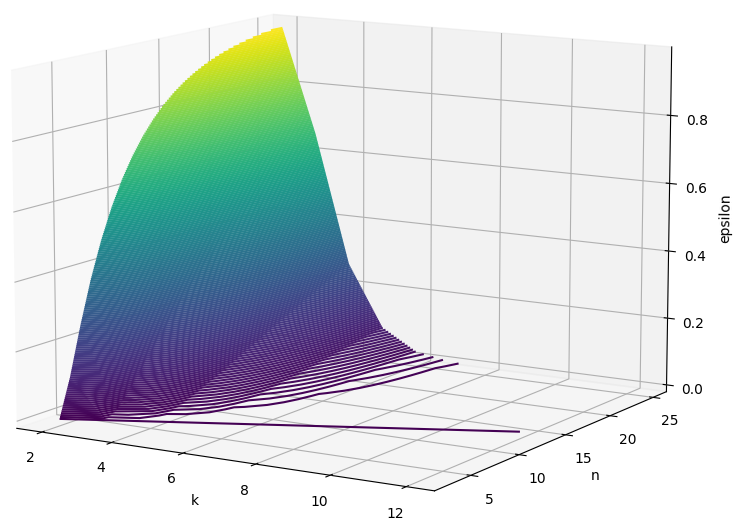
\includegraphics[width=16.5cm]{images/smallNoConsensusBetaOne.png}
    \end{figure*}
    \begin{figure*}
        Probability of not reaching consensus (β = 1) : -log(ε)
        \centering
        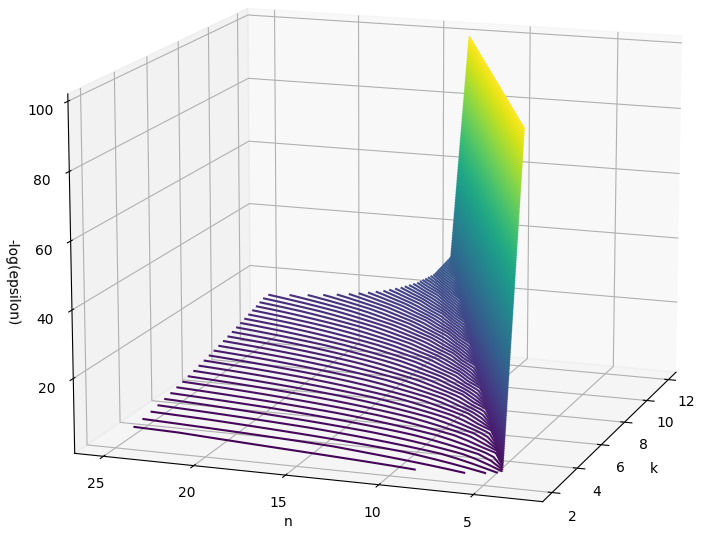
\includegraphics[width=16.5cm]{images/smalllogNoConsensusBetaOne.png}
    \end{figure*}
    \begin{figure*}
        Probability of not reaching consensus (β = 2) : ε
        \centering
        \includegraphics[width=16.5cm]{images/smallnoconsensus.png}
    \end{figure*}
    \begin{figure*}
        Probability of not reaching consensus (β = 2) : -log(ε)
        \centering
        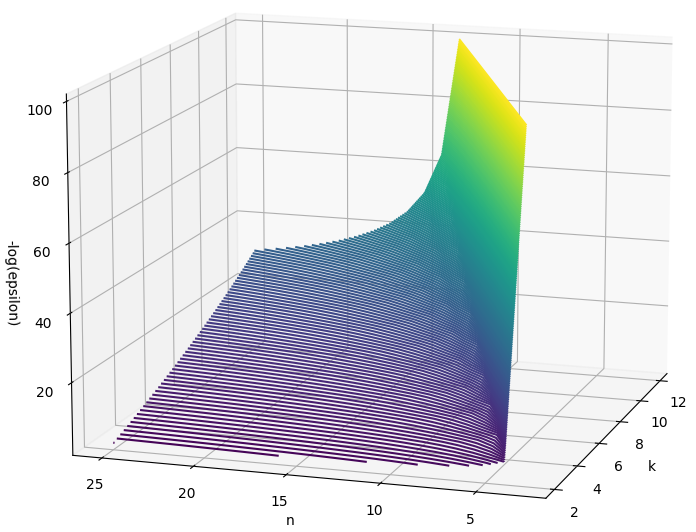
\includegraphics[width=16.5cm]{images/smalllognoconsensus.png}
    \end{figure*}
\end{appendices}
\end{document}
